%%%%%%%%%%%%%%%%%%%%%%%%%%%%%%%%%%%%%%%%%
% University/School Laboratory Report
% LaTeX Template
% Version 3.1 (25/3/14)
%
% This template has been downloaded from:
% http://www.LaTeXTemplates.com
%
% Original author:
% Linux and Unix Users Group at Virginia Tech Wiki 
% (https://vtluug.org/wiki/Example_LaTeX_chem_lab_report)
%
% License:
% CC BY-NC-SA 3.0 (http://creativecommons.org/licenses/by-nc-sa/3.0/)
%
%%%%%%%%%%%%%%%%%%%%%%%%%%%%%%%%%%%%%%%%%

%----------------------------------------------------------------------------------------
%	PACKAGES AND DOCUMENT CONFIGURATIONS
%----------------------------------------------------------------------------------------

\documentclass{article}

\usepackage[version=3]{mhchem} % Package for chemical equation typesetting
\usepackage{siunitx} % Provides the \SI{}{} and \si{} command for typesetting SI units
\usepackage{graphicx} % Required for the inclusion of images
\usepackage{natbib} % Required to change bibliography style to APA
\usepackage{amsmath} % Required for some math elements 

\usepackage{hyperref}
\hypersetup{
	colorlinks=true,
	linkcolor=blue,
	filecolor=magenta,      
	urlcolor=cyan,
}

\setlength\parindent{0pt} % Removes all indentation from paragraphs

\renewcommand{\labelenumi}{\alph{enumi}.} % Make numbering in the enumerate environment by letter rather than number (e.g. section 6)

%\usepackage{times} % Uncomment to use the Times New Roman font

%----------------------------------------------------------------------------------------
%	DOCUMENT INFORMATION
%----------------------------------------------------------------------------------------

\title{Comparison of \\ LTSpice and CircuitLab} % Title

\author{Pranav \textsc{Gade}} % Author name

\date{\today} % Date for the report

\begin{document}

\maketitle % Insert the title, author and date

\begin{center}
\begin{tabular}{l r}
Batch: & CS\&AI \\
Roll no.: & LCI2020010 \\
Date Performed: & December 1, 2020 \\ % Date the experiment was performed
Instructor: & Dr. Somesh Kumar % Instructor/supervisor
\end{tabular}
\end{center}

% If you wish to include an abstract, uncomment the lines below
% \begin{abstract}
% Abstract text
% \end{abstract}

%----------------------------------------------------------------------------------------
%	SECTION 1
%----------------------------------------------------------------------------------------

\section{Objective}

To study the interface and functions of electronic circuit simulator software LTSpice and CircuitLab.

% If you have more than one objective, uncomment the below:
%\begin{description}
%\item[First Objective] \hfill \\
%Objective 1 text
%\item[Second Objective] \hfill \\
%Objective 2 text
%\end{description}

\subsection{Components Required}
\label{definitions}
\begin{description}
\item[\href{https://www.circuitlab.com/}{Circuit Lab}]
CircuitLab is a browser-based circuit simulation and design program.
\item[\href{https://www.analog.com/en/design-center/design-tools-and-calculators/ltspice-simulator.html}{LTSpice}]
LTSpice is a SPICE\footnote{Simulation Program with Integrated Circuit Emphasis} based simulation and analysis program.
\end{description} 
 
%----------------------------------------------------------------------------------------
%	SECTION 2
%----------------------------------------------------------------------------------------

\section{Background}

\subsection{LTSpice}
LTSpice is currently the most popular circuit simulation software. It provides a schematic design and entry feature used to design or load predesigned circuits. Its primary feature, however, is simulating given circuits to verify their integrity and predict their behavior. Finally, the waveform viewer is another important feature available. Moreover, LTSpice offers much better performance when compared to other similar simulators. This dramatically reduces the time required to run simulations. \\
LTSpice offers a very stable platform, as well as a robust and intuitive schematics editor. This, coupled with the vast library of passive devices available, results in an unparalleled user experience, for beginners and experts alike.
\subsection{Circuit Lab}
Circuit Lab is a convenient and accessible alternative to LTSpice. Since it runs inside your browser, it requires minimal set-up and can be used on almost any device with a browser. This, however, comes at the cost of not being as sophisticated as LTSpice. One  can design schematics very easily using their intuitive editor, and generate professional PDFs, diagrams, and plots within seconds. Simulating digital as well as analog circuits can be done in seconds. One of the best features, however, is the share option. One can make a schematic public with a click, and share it with others.

%----------------------------------------------------------------------------------------
%	SECTION 3
%----------------------------------------------------------------------------------------

\section{Operation}

\subsection{LTSpice}
\begin{enumerate}
	\item When you open LTSpice, you can see the interface shown in fig. \ref{fig:ltspice_main}. The main components of this window are the menu bar, and the ribbon for quick access buttons, grouped by function.
	\begin{figure}[h]
		\centering
		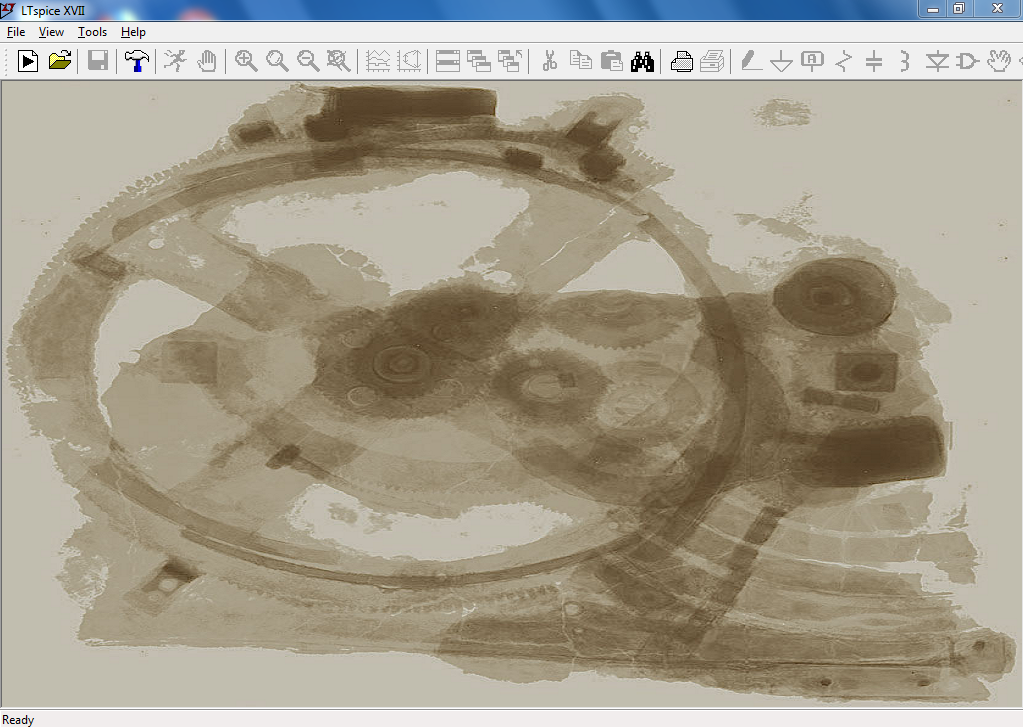
\includegraphics[width=0.7\linewidth]{Capture}
		\caption[Main Interface of LTSpice]{Main Interface of LTSpice}
		\label{fig:ltspice_main}
	\end{figure}
	\item Some notable tools included in the ribbon are load schematic, save, run, control buttons for navigating the schematic, and buttons for quick insertion of common components like resistors, capacitors, etc.
	\item After creating a new schematic, we can add components to make our circuit. Fig. \ref{fig:ltspice_2} shows an example arrangement, an LCR circuit.
	\begin{figure}[h]
		\centering
		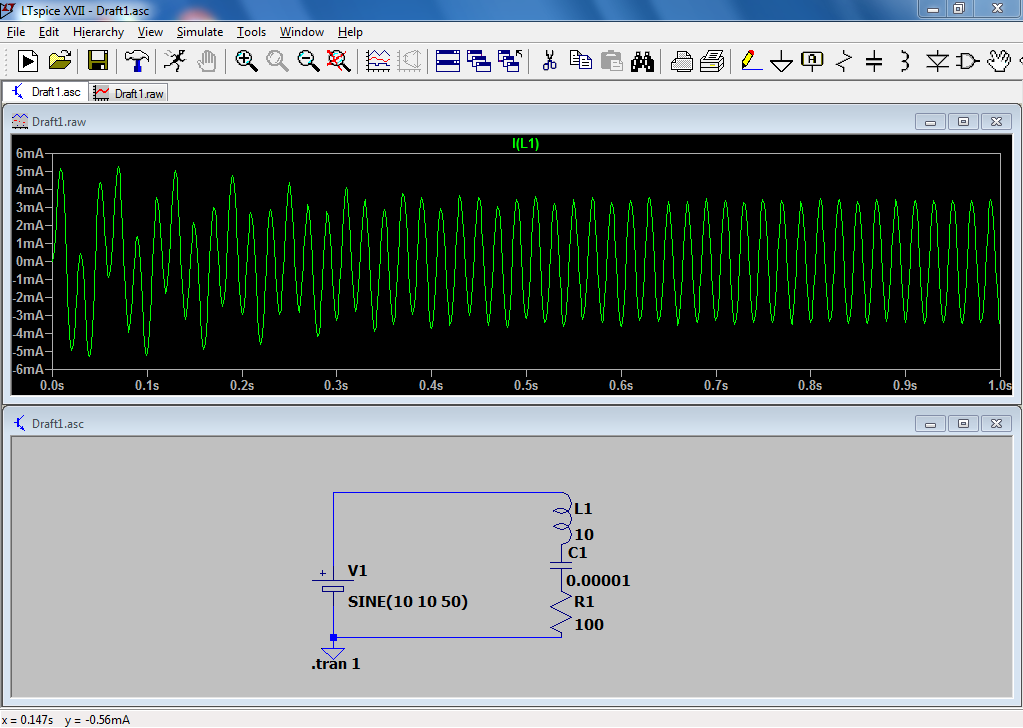
\includegraphics[width=0.7\linewidth]{Capture2}
		\caption{An LCR circuit and a graph of current through the inductor}
		\label{fig:ltspice_2}
	\end{figure}
	\item We can then run the simulation for an interval of our choice. After the simulation, we can probe any component to see its state through the simulation. Fig. \ref{fig:ltspice_2} shows the state of the inductor for an simulation interval of 1 second.
	\item We can also probe any two points on the circuit to look at the potential difference between them. Also, we can zoom into the graph wherever we like. We can see the graph of potential difference as well, zoomed in to include the first 200ms.
	\begin{figure}[h]
		\centering
		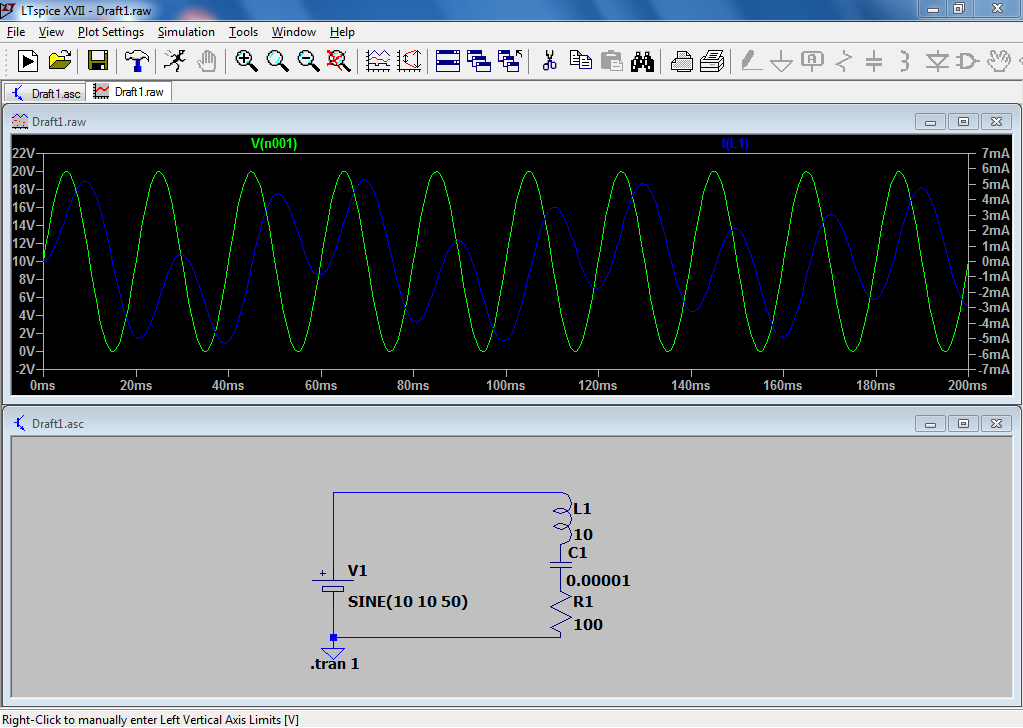
\includegraphics[width=0.7\linewidth]{Capture3}
		\caption{An LCR circuit with a graph of current as well as potential difference across the voltage source}
		\label{fig:ltspice_3}
	\end{figure}
	\item Finally, we can save the schematic for easier access at a later time, as well as for sharing the schematic.
\end{enumerate}

\subsection{Circuit Lab}
\begin{enumerate}
	\item When you go to \href{https://www.circuitlab.com}{circuitlab.com} and launch CircuitLab, you are taken to the interface shown in fig. \ref{fig:circuitlab}. The main components here are the side panel which gives you the components available to include in your circuit, the canvas, where you build your circuit, and the toolbar, where you have the buttons to run the simulation.
	\begin{figure}[h]
		\centering
		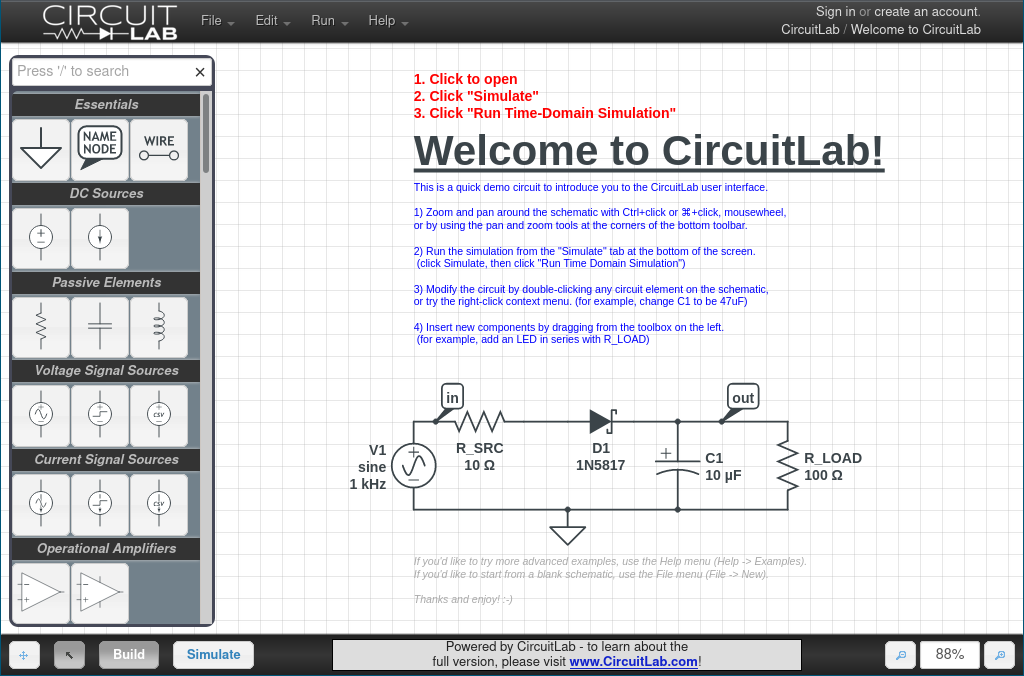
\includegraphics[width=0.7\linewidth]{circuitlab}
		\caption[CircuitLab interface]{CircuitLab interface}
		\label{fig:circuitlab}
	\end{figure}
	\item A lot of components are included in the side panel, grouped neatly according to function.
	\item We can create a new blank canvas, or start with the pre-made circuit. In this document, we will be discussing the latter. Fig. \ref{fig:circuitlab} shows the circuit.
	\item We can run the simulation with the parameters of our choice, as shown in fig. \ref{fig:simulation}. We can adjust the in and out probes, as seen in fig. \ref{fig:circuitlab} to choose the points where we would like to get the simulation results.
	\begin{figure}[h]
		\centering
		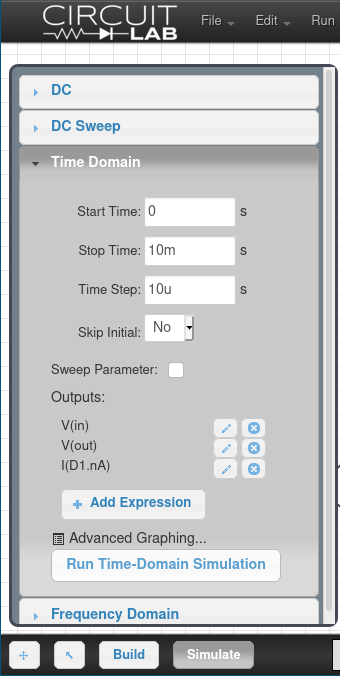
\includegraphics[width=5cm,height=5cm,keepaspectratio]{simulation}
		\caption[Simulation tab]{Simulation tab}
		\label{fig:simulation}
	\end{figure}
	\item After the simulation is run, we get the results as a graph as shown in fig. \ref{fig:graphs}. Similar to LTSpice, we can zoom in to specific sections of the graph for closer inspection.
	\begin{figure}[h]
		\centering
		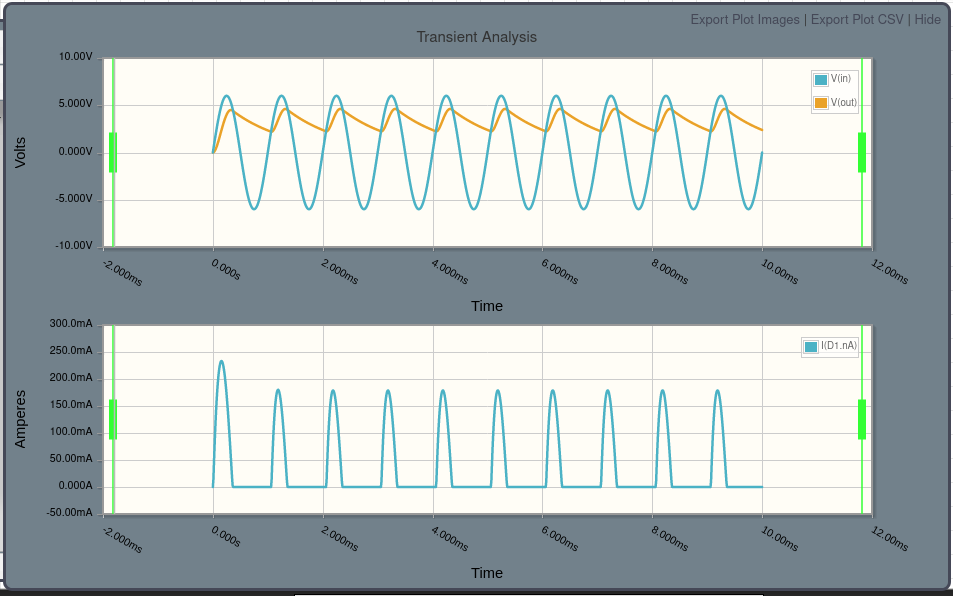
\includegraphics[width=0.7\linewidth]{graphs}
		\caption[Simulation results]{Simulation results}
		\label{fig:graphs}
	\end{figure}
	\item Finally, we can share the link of the circuit to others. Alternatively, we can save it in our account for future reference.


\end{enumerate}
\pagebreak
%----------------------------------------------------------------------------------------
%	SECTION 4
%----------------------------------------------------------------------------------------

\section{Conclusions}

After evaluating both LTSpice and CircuitLab, we can conclude that both have their pros and cons. They are summarized below:
\begin{itemize}
	\item LTSpice runs natively on your computer, and is therefore much faster for complex simulations.
	\item CircuitLab runs on all platforms, and makes sharing circuit designs very easy.
	\item The number of components and customizability LTSpice provides is vastly more than CircuitLab.
	\item Although CircuitLab provides graphs, they are limited compared to LTSpice, which can plot the state of individual components.
	\item Although both are freeware, LTSpice requires you to provide your details to sign up. Otherwise, you cannot run any simulations after 30 minutes.
\end{itemize}

\section{Results}
After careful evaluation of pro and cons of CircuitLab as well as LTSpice, I will be using LTSpice. This is partly due to the limits CircuitLab imposes, and partly due to the larger array of components included in LTSpice.

%----------------------------------------------------------------------------------------
%	BIBLIOGRAPHY
%----------------------------------------------------------------------------------------

\section*{References}
\renewcommand{\theenumi}{\arabic{enumi}}
\begin{itemize}
	\item \href{https://www.analog.com/en/design-center/design-tools-and-calculators/ltspice-simulator.html}{LTSpice website}
	\item \href{https://www.circuitlab.com/}{circuitlab.com}
\end{itemize}


%----------------------------------------------------------------------------------------


\end{document}